\documentclass[%
%draft,
11pt,%
twoside,%
titlepage,%
swissgerman,%
headsepline%
]{scrartcl}

\usepackage{lastpage}
\usepackage{amsthm}
\usepackage{amssymb}
\usepackage{geometry}
\usepackage{graphicx}
\usepackage[dvipsnames]{xcolor}
\usepackage[utf8]{inputenc}
\usepackage[swissgerman]{babel}
\usepackage{lscape}
\usepackage[framemethod=TikZ]{mdframed}
\usepackage[most]{tcolorbox}
\usepackage{enumerate}
\usepackage{units}
\usepackage{nicefrac}
\usepackage{pgf,tikz}
\usepackage{tikz-3dplot}
\usepackage{tkz-euclide}
\usetikzlibrary{arrows}
\usetikzlibrary{arrows.meta}
\usetikzlibrary{patterns}
\usetikzlibrary{positioning}
\usetikzlibrary{shadows}
\usetikzlibrary{quotes, angles}
\usepackage{colortbl}
\usepackage{hhline}
\usepackage{multirow}
\usepackage[extendedchars]{grffile}
\usepackage{caption}
\usepackage{multicol,calc}
\usepackage{blindtext}
\usepackage{pdfpages}
\usepackage{hyperref}
\usepackage{framed}

\usepackage{marginnote}
\usepackage{qrcode}
<<<<<<< Updated upstream
\qrset{height=9ex}
=======
\qrset{height=7ex}
>>>>>>> Stashed changes

\usepackage{longtable}
\usepackage{listings}
\usepackage{wrapfig}

\usepackage{fontawesome} % Oder FontAwesome, falls du ein Augensymbol aus einer
\newcommand{\faEyeLightGray}{\textcolor{lightgray}{\faEye}} % Custom command for the gray eye icon
\newcommand{\faReturnGray}{\textcolor{gray}{\faMailReply}} % Custom command for the gray eye icon
\usepackage{pifont} % weitere Zeichen
<<<<<<< Updated upstream
\usepackage{eurosym}
=======
>>>>>>> Stashed changes

% package für plots mit dem Befehl axes
\usepackage{pgfplots}



% Command, um Tabellen-Spalten anzupassen
\newcommand{\spaltenheight}{\rule{0mm}{3ex}}
\newcommand{\spaltenwidth}{\rule{3cm}{0mm}}
\newcommand{\spaltensep}{\\[1ex]}
%\arrayrulecolor{darkgreen}
\doublerulesepcolor{white}

% colors
\definecolor{lightyellow}{rgb}{1,1,0.8}
\definecolor{Gray}{gray}{0.9}
\definecolor{lightgray}{rgb}{0.7, 0.7, 0.7}
\definecolor{darkblue}{rgb}{0,0,0.55}
\definecolor{firebrick}{rgb}{0.7,0.13,0.13}
\definecolor{seagreen}{rgb}{0.18,0.55,0.34}
\definecolor{emerald}{HTML}{50C878} % color of Definition
\definecolor{whitesmoke}{HTML}{F5F5F5} % background for environments
\definecolor{myblizzardblue}{HTML}{87CEEB} % color of Satz

% Für Definitionen im Fliesstext
\newcommand{\definition}[1]{\colorbox{emerald}{#1}}
% Für Regeln im Fliesstext
\newcommand{\regel}[1]{\colorbox{myblizzardblue}{#1}}
% Für Merke/Achtungs im Fliesstext
\newcommand{\merke}[1]{\colorbox{firebrick}{#1}}
% Geogebra-Link
\newcommand{\geogebralink}{\href{https://www.geogebra.org/calculator}{\texttt{geogebra.org}}}

% Umgebungen
\theoremstyle{definition}
<<<<<<< Updated upstream
\newtheorem{bsp}{Beispiel}[subsection] % Beispiele
\newtheorem{bem}{Bemerkung}[subsection] % Bemerkungen
\theoremstyle{plain}
\newtheorem{thm}{Theorem} % Theorem [subsection]
\newtheorem{satz}{Satz} % Satz [subsection]
=======
    \newtheorem{bsp}{Beispiel}[subsection] % Beispiele
    \newtheorem{bem}{Bemerkung}[subsection] % Bemerkungen
\theoremstyle{plain}
    \newtheorem{thm}{Theorem} % Theorem [subsection]
    \newtheorem{satz}{Satz} % Satz [subsection]
>>>>>>> Stashed changes

% Umgebung lsg mit dynamischer Referenzierung und Label
\newcommand{\concatueb}[1]{ueb:#1}% Definition für concatueb
\newcommand{\concatlsg}[1]{lsg:#1}% Definition für concatlsg

\newcounter{uebcounter}[section]
\renewcommand{\theuebcounter}{\thesection.\arabic{uebcounter}}  % Zählerformat: Abschnitt.Übung

\newenvironment{lsg}[1]{%
<<<<<<< Updated upstream
	\par\noindent\textbf{Notizen zu Übung \theuebcounter\label{\concatlsg{#1}}}
	\hfill\hyperref[\concatueb{#1}]{\faReturnGray}\par % Hyperref-Button zurück zur Übung
}{%
	\par%
}

\newenvironment{uebenv}[1]{%
	\refstepcounter{uebcounter}
	\par\noindent\textbf{Übung \theuebcounter.}%
	\label{\concatueb{#1}}\hfill\hyperref[\concatlsg{#1}]{\faEyeLightGray}\par
}{%
	\par
=======
    \par\noindent\textbf{Notizen zu Übung \ref{\concatueb{#1}}}\label{\concatlsg{#1}}
    \hfill\hyperref[\concatueb{#1}]{\faReturnGray}\par % Hyperref-Button zurück zur Übung
}{%
    \par%
}

\newenvironment{uebenv}[1]{%
    \refstepcounter{uebcounter}
    \par\noindent\textbf{Übung \theuebcounter.}%
    \label{\concatueb{#1}}\hfill\hyperref[\concatlsg{#1}]{\faEyeLightGray}\par
}{%
    \par
>>>>>>> Stashed changes
}

% Umgebung für Definitionen
\newcounter{deff}[section]\setcounter{deff}{0}
\renewcommand{\thedeff}{\arabic{section}.\arabic{deff}}

\newenvironment{cdef}[1][]{%
<<<<<<< Updated upstream
	\refstepcounter{deff} 
	\ifstrempty{#1}%
	% if condition (without title)
	{\mdfsetup{%
			frametitle={%
				\tikz[baseline=(current bounding box.east),outer sep=0pt]
				\node[anchor=east,rectangle,fill=emerald]
				{\strut Definition~\thedeff};}
		}%
		% else condition (with title)
	}{\mdfsetup{%
			frametitle={%
				\tikz[baseline=(current bounding box.east),outer sep=0pt]
				\node[anchor=east,rectangle,fill=emerald]
				{\strut Definition~\thedeff:~#1};}%
		}%
	}%
	% for both conditions
	\mdfsetup{%
		innertopmargin=10pt,linecolor=emerald,%
		backgroundcolor=whitesmoke,%
		linewidth=2pt,topline=true,%
		frametitleaboveskip=\dimexpr-\ht\strutbox\relax%
	} 
	\begin{mdframed}[]\relax}{%
=======
    \refstepcounter{deff} 
    \ifstrempty{#1}%
    % if condition (without title)
    {\mdfsetup{%
        frametitle={%
            \tikz[baseline=(current bounding box.east),outer sep=0pt]
            \node[anchor=east,rectangle,fill=emerald]
            {\strut Definition~\thedeff};}
        }%
    % else condition (with title)
    }{\mdfsetup{%
        frametitle={%
            \tikz[baseline=(current bounding box.east),outer sep=0pt]
            \node[anchor=east,rectangle,fill=emerald]
            {\strut Definition~\thedeff:~#1};}%
        }%
    }%
% for both conditions
    \mdfsetup{%
        innertopmargin=10pt,linecolor=emerald,%
        backgroundcolor=whitesmoke,%
        linewidth=2pt,topline=true,%
        frametitleaboveskip=\dimexpr-\ht\strutbox\relax%
    } 
\begin{mdframed}[]\relax}{%
>>>>>>> Stashed changes
\end{mdframed}}

% Farbig umrahmte Umgebung Satz
\newcounter{satzz}[section]\setcounter{satzz}{0}
\renewcommand{\thesatz}{\arabic{section}.\arabic{satzz}}

\newenvironment{csatz}[1][]{%
<<<<<<< Updated upstream
	\refstepcounter{satzz}
	
	\ifstrempty{#1}%
	% if condition (without title)
	{\mdfsetup{%
			frametitle={%
				\tikz[baseline=(current bounding box.east),outer sep=0pt]
				\node[anchor=east,rectangle,fill=myblizzardblue]
				{\strut Satz~\thesatz};}
		}%
		% else condition (with title)
	}{\mdfsetup{%
			frametitle={%
				\tikz[baseline=(current bounding box.east),outer sep=0pt]
				\node[anchor=east,rectangle,fill=myblizzardblue]
				{\strut Satz~\thesatz:~#1};}%
		}%
	}%
	% for both conditions
	\mdfsetup{%
		innertopmargin=10pt,linecolor=myblizzardblue,%
		backgroundcolor=whitesmoke,%
		linewidth=2pt,topline=true,%
		frametitleaboveskip=\dimexpr-\ht\strutbox\relax%
	}
	\begin{mdframed}[]\relax}{%
=======
    \refstepcounter{satzz}
 
    \ifstrempty{#1}%
    % if condition (without title)
    {\mdfsetup{%
        frametitle={%
            \tikz[baseline=(current bounding box.east),outer sep=0pt]
            \node[anchor=east,rectangle,fill=myblizzardblue]
            {\strut Satz~\thesatz};}
        }%
    % else condition (with title)
    }{\mdfsetup{%
        frametitle={%
            \tikz[baseline=(current bounding box.east),outer sep=0pt]
            \node[anchor=east,rectangle,fill=myblizzardblue]
            {\strut Satz~\thesatz:~#1};}%
        }%
    }%
% for both conditions
    \mdfsetup{%
        innertopmargin=10pt,linecolor=myblizzardblue,%
        backgroundcolor=whitesmoke,%
        linewidth=2pt,topline=true,%
        frametitleaboveskip=\dimexpr-\ht\strutbox\relax%
    }
\begin{mdframed}[]\relax}{%
>>>>>>> Stashed changes
\end{mdframed}}

% kein Einzug bei neuem Abschnitt
\setlength{\parindent}{0pt} \setlength{\parskip}{1em}
\pagestyle{headings} % gemachte Einstellungen anwenden

<<<<<<< Updated upstream
=======

>>>>>>> Stashed changes
\subject{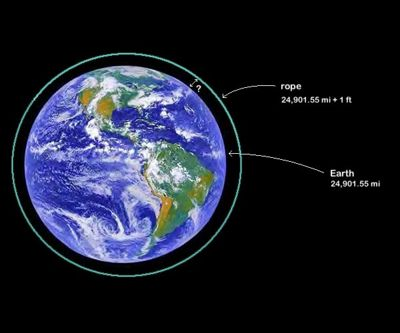
\includegraphics[width=0.618\textwidth]{pictures/rope}}
\title{Lineare Funktionen und Optimierung}
\subtitle{\dots und der Differenzenquotient}
\author{}
\date{}
\lowertitleback{
	
\includegraphics[height=1cm]{pictures/gymfmslerbermattlogo.eps}
	\hfill%\copyright%
	{\begin{tikzpicture}
			% Draw the rounded rectangle and clip the image to it
			\clip [rounded corners=5mm] (0,0) rectangle (1,1); % Adjust dimensions as needed
			\node at (0.5,0.5) {\includegraphics[width=1cm]{pictures/teacher_me_caricatur.png}}; % Adjust width and center image
	\end{tikzpicture}}
}

\begin{document}
	\maketitle
	\tableofcontents
	%\thispagestyle{empty}
	\cleardoublepage
	%\setcounter{page}{1}
	
	\section{Funktionen}
	\subsection{Grundlagen}
	Aus dem Alltag kennen Sie graphische Darstellungen von Funktionen. Zum Beispiel wird in den Nachrichten der SMI (Swiss Market Index) häufig als Graph illustriert.
	\begin{bsp}
		
		\begin{center}
			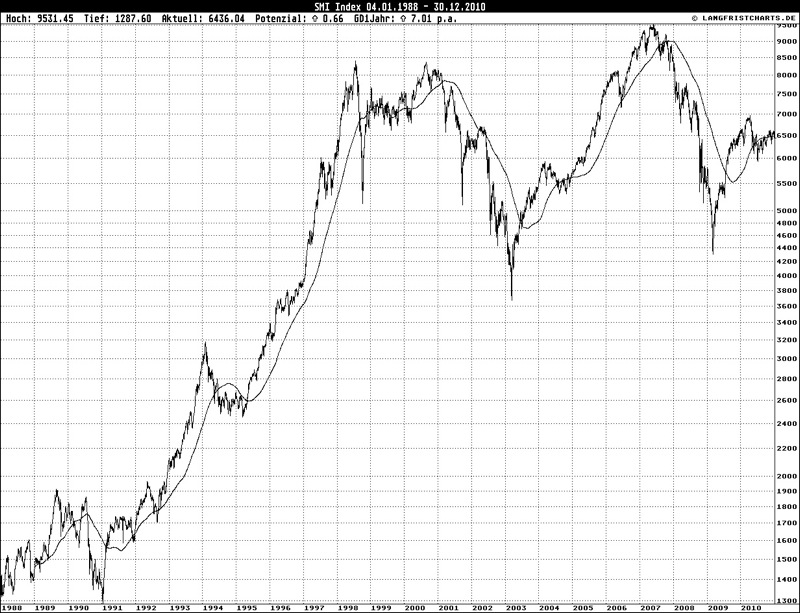
\includegraphics[width=0.7\textwidth]{pictures/smi}
		\end{center}
		
		Jedem Datum wird ein bestimmter Index zugeordnet.
		
	\end{bsp}
	In der Mathematik versteht man unter einer Funktion folgendes.
	
	\begin{cdef}[Funktion]
		Eine Funktion ist eine Zuordnung, bei der jedem Element $x$ einer Menge $\mathbb{D}$ eindeutig ein Element $y$ einer Menge $\mathbb{W}\subseteq\mathbb{R}$ zugeordnet wird. Man schreibt: $$y=f(x)$$
		(sprich:\glqq $y$ gleich $f$ von $x$\grqq)
	\end{cdef}
	
	Anschaulich stellt man eine Funktion mit Mengendiagrammen dar.
	
	\begin{cdef}[Argument]
		Die Menge $\mathbb{D}$ nennt man \definition{Definitionsmenge}. Ein Element $x\in\mathbb{D}$ heisst Argument von $f$ oder neudeutsch input. $x$ wird auch als unabhängige Variable bezeichnet.
	\end{cdef}
	
	\begin{cdef}[Funktionswert]
		Die Menge $\mathbb{W}$ nennt man \definition{Wertemenge} oder Bildmenge von $f$.  Ein Element $y\in\mathbb{W}$ heisst Funktionswert oder neudeutsch output. $y$ wird auch häufig als abhängige Variable bezeichnet.
	\end{cdef}
	
	\begin{bsp}
		Beim SMI ordnet die Funktion $f$ jedem Monat $x$ genau eine Quote $y$ zu.
	\end{bsp}
	
	\begin{bsp}
		Das Quadrieren ist eine Funktion. Jeder reellen Zahl $x$ wird ihr Quadrat
		$$y=x^2$$
		zugeordnet.
	\end{bsp}
	
	\subsection{Darstellungen}
	
	Will man beispielsweise als Funktion das Quadrieren --- hier am Beispiel der Werte $-2,-1,0,1,2$ --- darstellen, so kann dies auf verschiedene Arten geschehen:
	
	\begin{itemize}
		\item Schreibweise konkret mit Funktionswerte:
		$f(-2)=4$, $f(-1)=1$, $f(0)=0$, $f(1)=1, f(2)=4$
		\item Darstellung als Wertetabelle:
		\begin{center}
			\renewcommand{\arraystretch}{1.2}
			\begin{tabular}{c | rrrrr}
				$x$ & $-2$ &$-1$ & $0$ & $1$ & $2$ \\
				\hline
				$y$ & $4$ & $1$ & $0$ & $1$ & $4$
			\end{tabular}
		\end{center}
		
		\item Darstellung als Funktionsgleichung:
		$$f(x)=x^2,\quad\mathbb{D}=\{-2,-1,0,1,2\}$$
		
		\item graphische Darstellung in einem Koordinatensystem:
		
		\begin{figure}[h!]
			\begin{center}
				\begin{tikzpicture}[line cap=round,line join=round, x=0.8cm,y=0.8cm]
					\draw[-{Latex[length=8pt, width=8pt]},color=black] (-4.46,0) -- (5,0);
					\foreach \x in {-4,-3,-2,-1,1,2,3,4}
					\draw[shift={(\x,0)},color=black] (0pt,2pt) -- (0pt,-2pt) node[below] {\footnotesize $\x$};
					\draw[color=black] (4.69,0.06) node [anchor=south west] {$x$};
					\draw[-{Latex[length=8pt, width=8pt]},color=black] (0,-1.5) -- (0,4.49);
					\foreach \y in {-1,1,2,3,4}
					\draw[shift={(0,\y)},color=black] (2pt,0pt) -- (-2pt,0pt) node[left] {\footnotesize $\y$};
					\draw[color=black] (0.07,4.19) node [anchor=west] {$y$};
					\draw[color=black] (0pt,-10pt) node[right] {\footnotesize $0$};
					\clip(-4.46,-1.5) rectangle (4.92,4.49);
					\draw [line width=1.1pt,dotted,lightgray] (-2,4)-- (0,4);
					\draw [line width=1.1pt,dotted,lightgray] (-2,4)-- (-2,0);
					\draw (-3.02,4.7) node[anchor=north] {$(-2\mid 4)$};
					\fill [color=black] (-2,4) circle (1.5pt);
					\fill [color=black] (-1,1) circle (1.5pt);
					\fill [color=black] (0,0) circle (1.5pt);
					\fill [color=black] (1,1) circle (1.5pt);
					\fill [color=black] (2,4) circle (1.5pt);
				\end{tikzpicture}
			\end{center}
			\caption{Graphische Darstellung im Koordinatensystem}
		\end{figure}
	\end{itemize}
	
	\subsection{Graph einer Funktion}
	
	\begin{cdef}[Geordnetes Paar]
		Ein Paar $(x\mid y)$ heisst geordnet, wenn die Reihenfolge von $x$ und $y$ wesentlich ist.
	\end{cdef}
	
	\begin{cdef}[Graph]
		Sei $f:\mathbb{D}\longrightarrow\mathbb{W}$ eine Funktion. Die Menge aller geordneten Paare
		$$G_f=\{(x\mid  f(x))\mid x\in\mathbb{D}\}$$
		heisst Graph von $f$.
	\end{cdef}
	
	\subsection{Einschränkungen des Definitionsbereichs einer Funktion}
	
	Für manche Beschreibungen von alltäglichen Zusammenhängen, die als Funktionen beschrieben werden, ist die Anpassung der Definitionsmenge der entsprechenden Funktion sinnvoll. Im Folgenden wird der Einfluss der Definitionsmenge auf die Funktion bzw. ihren Graphen veranschaulicht.
	
	\begin{bsp}
		Wir betrachten den Graphen der Funktion
		$$f(x)=x^2$$
		für verschiedene Definitionsmengen.
		
		\begin{center}
			\begin{figure}[h!]
				\centering
				\scalebox{1}{
					\begin{tikzpicture}[line cap=round,line join=round, x=0.7cm,y=0.7cm]
						\draw[-{Latex[length=8pt, width=8pt]},color=black] (-3.28,0) -- (3.22,0);
						\foreach \x in {-3,-2,-1,1,2,3}
						\draw[shift={(\x,0)},color=black] (0pt,2pt) -- (0pt,-2pt) node[below] {\footnotesize $\x$};
						\draw[color=black] (2.99,0.06) node [anchor=south west] {$x$};
						\draw[-{Latex[length=8pt, width=8pt]},color=black] (0,-0.9) -- (0,6.65);
						\foreach \y in {,1,2,3,4,5,6}
						\draw[shift={(0,\y)},color=black] (2pt,0pt) -- (-2pt,0pt) node[left] {\footnotesize $\y$};
						\draw[color=black] (0.07,6.35) node [anchor=west] {$y$};
						\draw[color=black] (0pt,-10pt) node[right] {\footnotesize $0$};
						\clip(-3.28,-0.9) rectangle (3.22,6.65);
						\draw[line width=1.5pt,seagreen, smooth,samples=100,domain=-3.285:3.2225] plot(\x,{(\x)^2});
					\end{tikzpicture}
				}
				\caption{$f:\mathbb{R}\longrightarrow\mathbb{R}$}
			\end{figure}
		\end{center}
		\begin{center}
			\begin{figure}[h!]
				\centering
				\scalebox{1}{
					\begin{tikzpicture}[line cap=round,line join=round, x=0.7cm,y=0.7cm]
						\draw[-{Latex[length=8pt, width=8pt]},color=black] (-3.28,0) -- (3.22,0);
						\foreach \x in {-3,-2,-1,1,2,3}
						\draw[shift={(\x,0)},color=black] (0pt,2pt) -- (0pt,-2pt) node[below] {\footnotesize $\x$};
						\draw[color=black] (2.99,0.06) node [anchor=south west] { x};
						\draw[-{Latex[length=8pt, width=8pt]},color=black] (0,-0.9) -- (0,6.65);
						\foreach \y in {,1,2,3,4,5,6}
						\draw[shift={(0,\y)},color=black] (2pt,0pt) -- (-2pt,0pt) node[left] {\footnotesize $\y$};
						\draw[color=black] (0.07,6.35) node [anchor=west] { y};
						\draw[color=black] (0pt,-10pt) node[right] {\footnotesize $0$};
						\clip(-3.28,-0.9) rectangle (3.22,6.65);
						\fill [color=seagreen] (-1,1) circle (2.0pt);
						\fill [color=seagreen] (-2,4) circle (2.0pt);
						\fill [color=seagreen] (0,0) circle (2.0pt);
						\fill [color=seagreen] (1,1) circle (2.0pt);
						\fill [color=seagreen] (2,4) circle (2.0pt);
					\end{tikzpicture}
				}
				\caption{$f:\mathbb{Z}\longrightarrow\mathbb{R}$}
			\end{figure}
		\end{center}
		\begin{center}
			\begin{figure}[h!]
				\centering
				\scalebox{1}{
					\begin{tikzpicture}[line cap=round,line join=round, x=0.7cm,y=0.7cm]
						\draw[-{Latex[length=8pt, width=8pt]},color=black] (-3.28,0) -- (3.22,0);
						\foreach \x in {-3,-2,-1,1,2,3}
						\draw[shift={(\x,0)},color=black] (0pt,2pt) -- (0pt,-2pt) node[below] {\footnotesize $\x$};
						\draw[color=black] (2.99,0.06) node [anchor=south west] { x};
						\draw[-{Latex[length=8pt, width=8pt]},color=black] (0,-0.9) -- (0,6.65);
						\foreach \y in {,1,2,3,4,5,6}
						\draw[shift={(0,\y)},color=black] (2pt,0pt) -- (-2pt,0pt) node[left] {\footnotesize $\y$};
						\draw[color=black] (0.07,6.35) node [anchor=west] { y};
						\draw[color=black] (0pt,-10pt) node[right] {\footnotesize $0$};
						\clip(-3.28,-0.9) rectangle (3.22,6.65);
						\fill [color=black] (1,1) circle (2.0pt);
						\fill [color=black] (2,4) circle (2.0pt);
					\end{tikzpicture}
				}
				\caption{$f:\mathbb{N}\longrightarrow\mathbb{R}$}
			\end{figure}
		\end{center}
	\end{bsp}
	
	\begin{uebenv}{gerade}
		Gegeben sei die Funktion
		$$f(x)=-x+2.$$
		\begin{enumerate}[a)]
			\item Berechne $f(1),f(0)$ und $f(-1)$.
			\item Zeichne den Graphen für
			\begin{enumerate}[i)]
				\item $f:\mathbb{R}\rightarrow\mathbb{R}$
				\item und für $f:\mathbb{N}\rightarrow\mathbb{R}$
			\end{enumerate}
		\end{enumerate}
	\end{uebenv}
	
	\begin{uebenv}{xhochdrei}
		Sei $f(x)=x^3$.
		Berechne einige Funktionswerte und skizziere den Graphen.
	\end{uebenv}
	
	\begin{uebenv}{freierfall}
		Gegeben sei die Funktion
		$$s(t)=20-5t^2.$$
		\begin{enumerate}[a)]
			\item Berechne $s(-1),s(0)$ und $s(1)$.
			\item Wann gilt $s(t)=0$?
			\item Bestimme
			\begin{enumerate}[i)]
				\item $s(2)-s(1)$
				\item $\frac{s(3)-s(1)}{3-1}$
				\item $\frac{s(1+h)-s(1)}{h}$
			\end{enumerate}
			\item Berechne allgemein für beliebiges $t$ den Quotienten
			$$\frac{s(t+h)-s(t)}{h}$$
			und überlege dir, welchen Wert dieser Quotient für $h\to0$ annehmen müsste.
		\end{enumerate}
	\end{uebenv}
	
	\begin{uebenv}{exponentiell}
		Man weiss von einer Funktion vom Typ
		$$N(t)=a\cdot b^t,$$
		dass sie die Werte $N(0)=10$ und $N(2)=6.4$ annimmt.
		\begin{enumerate}[a)]
			\item Bestimme die Parameter $a$ und $b$.
			\item Berechne $N(1)$ und $N(-2)$.
			\item Skizziere den Graphen.
			\item Bestimme
			\begin{enumerate}[i)]
				\item $\frac{N(2)-N(0)}{2}$
				\item $\frac{N(3)-N(1)}{2}$
				\item $\frac{N(t+h)-N(t)}{h}$
			\end{enumerate}
		\end{enumerate}
	\end{uebenv}

\clearpage

\subsection{Notizen zu den Übungen}
	
	\begin{lsg}{gerade}
		\begin{enumerate}[a)]
			\item $f(1)=1,f(0)=2$ und $f(-1)=3$.
			\item
			\begin{enumerate}[i)]
				\item Für $x\in\mathbb{R}$:
				
				\begin{tikzpicture}
					\draw[step=1cm,gray,very thin] (-0.5,-0.5) grid (2.5,2.5);
					\draw[-{Latex[length=8pt, width=8pt]}] (-1,0) -- (3,0) node[right] {$x$};
					\draw[-{Latex[length=8pt, width=8pt]}] (0,-1) -- (0,3) node[above] {$f(x)$};
					\draw[domain=-1:2.5, smooth, variable=\x, seagreen, thick] plot ({\x},{-1*\x + 2});
					\node[below left] at (2,0) {$2$};
					\node[below left] at (0,2) {$2$};
					\node[below left] at (0,0) {$0$};
				\end{tikzpicture}
				\item \begin{tikzpicture}
					\draw[step=1cm,gray,very thin] (-0.5,-1.5) grid (3.5,2.5);
					\draw[-{Latex[length=8pt, width=8pt]}] (-2,0) -- (4,0) node[right] {$x$};
					\draw[-{Latex[length=8pt, width=8pt]}] (0,-1) -- (0,3) node[above] {$f(x)$};
					\foreach \x in {1,2,3} {
						\draw[fill, seagreen] (\x,{-\x + 2}) circle [radius=0.05];
					}
					\node[above left] at (0,1) {$1$};
					\node[below left] at (0,0) {$0$};
					\node[below left] at (2,0) {$2$};
				\end{tikzpicture}
			\end{enumerate}
		\end{enumerate}
	\end{lsg}
	\begin{lsg}{xhochdrei}
		Bekanntlich sind meine Favoriten $f(0)=0$, $f(1)=1$ und $f(-1)=-1$. Ferner berechne ich noch $f(2)=8$, $f(\frac{1}{2})=\frac{1}{8}$. Der Plot sieht so aus:
		
		\begin{tikzpicture}
			\begin{axis}[
				domain=-1.5:1.5,
				samples=100,
				axis lines=middle,
				xlabel={$x$},
				ylabel={$f(x)$},
				grid=both,
				width=10cm,
				height=10cm,
				enlargelimits=true,
				xtick={-1.5,-1,...,1.5},
				ytick={-3,-2,...,3}
				]
				\addplot[seagreen, thick] {x^3};
			\end{axis}
		\end{tikzpicture}
	\end{lsg}
	\begin{lsg}{freierfall}
		\begin{enumerate}[a)]
			\item $s(-1)=20-5\cdot(-1)^2=15$, $s(0)=20$, $s(1)=15$.
			\item $20-5t^2\stackrel{!}{=}0\Leftrightarrow t=\pm2$
			\item $s(2)-s(1)=0-15=-15$, $\frac{s(3)-s(1)}{3-1}=\frac{-25-15}{2}=-20$, und 
			\begin{align*}
				\frac{s(1+h)-s(1)}{h} &= \frac{20-5(1+h)^2-15}{h}=\frac{20-(5+10h+5h^2)-15}{h}=\frac{-10h-5h^2}{h}\\
				&= -10-5h
			\end{align*}
			\item
			\begin{align*}
				\frac{s(t+h)-s(t)}{h} &= \frac{20-5(t+h)^2-(20-5t^2)}{h} = \frac{20-5t^2-10th-5h^2-20+5t^2}{h}\\
				&= \frac{-10th-5h^2}{h}=-10t-5h
			\end{align*}
			Der Quotient strebt für $h\to0$ gegen $-10t$.
		\end{enumerate}
	\end{lsg}
	\begin{lsg}{exponentiell}
		\begin{enumerate}[a)]
			\item Wegen $N(0)=10=a$ und daraus $N(2)=10b^2=6.4\Leftrightarrow b^2=0.64\Leftrightarrow b=\pm0.8$. $b$ wird positiv gewählt wegen der Definitheit.
			\item $N(1)=10\cdot0.8^1=8$ und $N(-2)=10\cdot0.8^{-2}=10\cdot 64=640$.
			\item Deine Skizze vergleichst du mit \geogebralink.
			\item Exemplarisch $\frac{N(2)-N(0)}{2}=\frac{6.4-10}{2}=-1.8$ und $\frac{N(t+h)-N(t)}{h}=\frac{10\cdot0.8^t(0.8^h-1)}{h}$
		\end{enumerate}
	\end{lsg}
	
	\pagebreak
	
	\section{Proportionalität}
	%\begin{wrapfigure}{r}{0.382\textwidth}
	\begin{center}
		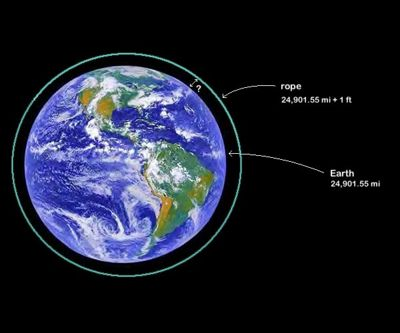
\includegraphics[width=0.618\textwidth]{pictures/rope}
	\end{center}
	%\caption{A gull}
	%\end{wrapfigure}
	Wir betrachten eine spezielle Menge von Funktionen, die Proportionalitäten und umgekehrten Proportionalitäten.
	\begin{cdef}[Proportionalität]
		Eine Funktion der Form
		$$f(x)=mx\quad m\in\mathbb{R}$$
		heisst Proportionalität. Der Parameter $m$ heisst Proportionalitätskonstante oder Proportionalitätsfaktor.
	\end{cdef}
	\begin{bsp}
		Die Menge der nötigen Zutaten für ein Rezept in Abhängigkeit der Anzahl Essenden ist eine Proportionalität. (Spätzle-Eintopf)
	\end{bsp}
	
	\begin{csatz}[Charakteristik]
		Die zu einer Proportionalität $f$ gehörenden Zahlenpaare haben denselben Quo\-tien\-ten.
	\end{csatz}
	
	\begin{proof}
		Sei $f(x)=mx$ eine Proportionalität. Dann gilt für beliebige Zahlenpaare
		$$(x\mid y)=(x\mid mx)$$
		und damit für den Quotienten
		$$\frac{y}{x}=\frac{mx}{x}=m$$
	\end{proof}
	
	
	\begin{bsp}
		Der Schweredruck $P$ unter Wasser ist proportional zur Tiefe $h$ unter der Wasseroberfläche. Aus der Physik kennt man die Beziehung
		$$P(h)=\rho_wgh$$
		wobei $\rho_w$ die Dichte von Wasser und $g$ den Ortsfaktor bezeichnet. $P(h)$ ist eine Proportionalität mit Proportionalitätskonstante $\rho_wg$.
	\end{bsp}
	
	\begin{bem}
		Wenn für die Argumentation bloss wichtig ist, dass es sich um eine Proportionalität handelt und der Wert der Konstanten keine Rolle spielt, schreibt man kurz \glqq$\sim$\grqq. Im obigen Beispiel würde man kurz schreiben
		$$P\sim h$$
	\end{bem}
	
	\section{Lineare Funktionen}
	
	In diesem Abschnitt werden wir die Menge der Proportionalitäten erweitern.
	
	\begin{bsp}
		Für ein Handy-Abonnement zahlt man eine Grundgebühr von $\unit[10]{Franken}$ pro Monat. Jede SMS kostet den Abonnementen $\unit[25]{Rappen}$. Wir stellen die anfallenden Kosten in Abhängigkeit der verschickten SMS dar. Dabei gehen wir schrittweise vor und wählen der Einfachheit halber als Defini\-tions\-menge $\mathbb{D}=\mathbb{R}^+_0$.
		
		\begin{enumerate}[a)]
			\item Würde man keine Grundgebühr zahlen, sondern nur die versendeten SMS, dann lautete die Kostenfunktion (Einheiten in Franken)
			$$f(x)=0.25x.$$
			\begin{center}
				\scalebox{0.9}{
					\begin{tikzpicture}[line cap=round,line join=round, x=0.3cm,y=0.3cm]
						\draw [color=lightgray,dash pattern=on 2pt off 2pt, xstep=0.6cm,ystep=0.6cm] (-1.56,-1.34) grid (18.4,15);
						\draw[-{Latex[length=8pt, width=8pt]},color=black] (-1.56,0) -- (18.4,0);
						\foreach \x in {,2,4,6,8,10,12,14,16,18}
						\draw[shift={(\x,0)},color=black] (0pt,2pt) -- (0pt,-2pt) node[below] {\footnotesize $\x$};
						\draw[color=black] (17.52,0.1) node [anchor=south west] { \# SMS};
						\draw[-{Latex[length=8pt, width=8pt]},color=black] (0,-1.34) -- (0,15);
						\foreach \y in {,2,4,6,8,10,12,14}
						\draw[shift={(0,\y)},color=black] (2pt,0pt) -- (-2pt,0pt) node[left] {\footnotesize $\y$};
						\draw[color=black] (0.1,14.48) node [anchor=west] { Kosten};
						\draw[color=black] (0pt,-10pt) node[right] {\footnotesize $0$};
						\clip(-1.56,-1.34) rectangle (18.4,15);
						\draw[line width=1.5pt, smooth,samples=100,domain=0.0:18.4, seagreen] plot(\x,{0.25*\x});
						\draw[color=seagreen] (4,2) node {$f$};
					\end{tikzpicture}
				}
			\end{center}
			\item Mit Grundgebühr erhalten wir die Kostenfunktion
			$$k(x)=0.25x+10$$
			\begin{center}
				\scalebox{0.9}{
					\begin{tikzpicture}[line cap=round,line join=round, x=0.3cm,y=0.3cm]
						\draw [color=lightgray,dash pattern=on 2pt off 2pt, xstep=0.6cm,ystep=0.6cm] (-1.56,-1.34) grid (18.4,15);
						\draw[-{Latex[length=8pt, width=8pt]},color=black] (-1.56,0) -- (18.4,0);
						\foreach \x in {,2,4,6,8,10,12,14,16,18}
						\draw[shift={(\x,0)},color=black] (0pt,2pt) -- (0pt,-2pt) node[below] {\footnotesize $\x$};
						\draw[color=black] (17.52,0.1) node [anchor=south west] { \# SMS};
						\draw[-{Latex[length=8pt, width=8pt]},color=black] (0,-1.34) -- (0,15);
						\foreach \y in {,2,4,6,8,10,12,14}
						\draw[shift={(0,\y)},color=black] (2pt,0pt) -- (-2pt,0pt) node[left] {\footnotesize $\y$};
						\draw[color=black] (0.1,14.48) node [anchor=west] { Kosten};
						\draw[color=black] (0pt,-10pt) node[right] {\footnotesize $0$};
						\clip(-1.56,-1.34) rectangle (18.4,15);
						\draw[line width=1.5pt, smooth,samples=100,domain=0.0:18.4, firebrick] plot(\x,{0.25*\x+10});
						\draw[color=firebrick] (1.6,11.4) node {$k$};
					\end{tikzpicture}
				}
			\end{center}
		\end{enumerate}
	\end{bsp}
	
	Im vorangegangenen Beispiel sieht man, dass die Addition der Grundgebühr eine Verschiebung des Graphen parallel zur $y$-Achse um $10$ bewirkt:
	$$k(x)=0.25x+10=f(x)+10$$
	
	\subsection{Mathematische Beschreibung}
	\begin{cdef}[Lineare Funktion]
		Eine Funktion der Form
		$$f(x)=mx+b\quad m,b\in\mathbb{R}$$
		heisst linear. Den Parameter $m$ nennt man \definition{Steigung}, den Parameter $b$ Ordinatenabschnitt oder \definition{$y$-Achsenabschnitt}.
	\end{cdef}
	
	\begin{csatz}[Gerade]
		Der Graph einer affinen Funktion
		$$f(x)=mx+b$$
		ist eine Gerade, die die $y$-Achse bei $b$ schneidet.
	\end{csatz}
	
	\begin{proof}
		Dass der Graph eine Gerade ist überlegt man sich mit einem einfachen Ähnlichkeitsargument basierend auf der Steigung. Der $y$-Achsen-Schnittpunkt liegt wegen
		$$f(0)=m\cdot0+b=b$$
		im Punkt $(0\mid b)$.
	\end{proof}
	
	\begin{figure}[h!]
		\begin{center}
			\scalebox{0.8}{
				\begin{tikzpicture}[line cap=round,line join=round, x=0.6cm,y=0.6cm]
					\draw[-{Latex[length=8pt, width=8pt]},color=black] (-3,0) -- (7.47,0);
					\foreach \x in {-2,2,4,6}
					\draw[shift={(\x,0)},color=black] (0pt,2pt) -- (0pt,-2pt);
					\draw[color=black] (7.21,0.08) node [anchor=south west] {$x$};
					\draw[-{Latex[length=8pt, width=8pt]},color=black] (0,-1) -- (0,7.83);
					\foreach \y in {2,4,6}
					\draw[shift={(0,\y)},color=black] (2pt,0pt) -- (-2pt,0pt);
					\draw[color=black] (0.08,7.42) node [anchor=west] {$y$};
					\clip(-2.68,-1.3) rectangle (7.47,7.83);
					\draw[line width=2pt, smooth,samples=100,domain=-2.6829:7.47085,seagreen] plot(\x,{0.5*\x+3});
					\draw (0,3)-- (0.36,3);
					\draw [line width=1.6pt, darkblue] (0.21,3)-- (0.21,0);
					\draw [line width=1.6pt] (2,4)-- (4,4);
					\draw [line width=1.6pt,firebrick] (4,4)-- (4,5);
					\draw (2.95,4) node[anchor=north west] {$1$};
					\draw (4.1,4.7) node[anchor=north west,firebrick] {$m$};
					\draw[color=darkblue] (0.5,1.61) node {$b$};
				\end{tikzpicture}
			}
		\end{center}
		\caption{Steigung und y-Achsen-Abschnitt}
	\end{figure}
	
	\begin{bem}
		Weil der Graph einer affinen Funktion eine Gerade ist, reichen zwei Punkte um dessen Funktionsgleichung bestimmen zu können bzw. um dessen Graphen skizzieren zu können.
	\end{bem}
	
	\subsection{Funktionsgleichung aus zwei gegebenen Punkten bestimmen}
	
	\begin{bsp}
		Wir bestimmen die Funktionsgleichung der Geraden, die durch die Punkte $P=(-1\mid 1)$ und $Q=(3\mid 2)$ geht. Weil der Graph eine Gerade ist, muss ihre Funktionsgleichung die Form
		$$f(x)=mx+b$$
		haben.
		
		Die Differenz der $x$-Werte der beiden Punkte ist $q_x-p_x=3-(-1)=4$ und die der $y$-Werte $q_y-p_y=2-1=1$. Daher ergibt sich für die Steigung
		$$m=\frac{\text{Höhendifferenz}}{\text{Strecke horizontal}}=\frac{q_y-p_y}{q_x-p_x}=\frac{1}{4}.$$
		\begin{center}
			\scalebox{1.0}{
				\begin{tikzpicture}[line cap=round,line join=round, x=1.1cm,y=1.1cm]
					\draw [color=lightgray,dash pattern=on 1.5pt off 1.5pt, xstep=1.1cm,ystep=1.1cm] (-1.5,-1.4) grid (4.6,2.8);
					\draw[-{Latex[length=8pt, width=8pt]},color=black] (-2,0) -- (4.6,0);
					\foreach \x in {-2,-1,1,2,3,4}
					\draw[shift={(\x,0)},color=black] (0pt,2pt) -- (0pt,-2pt) node[below] {\footnotesize $\x$};
					\draw[color=black] (4.5,0.08) node [anchor=south west] {$x$};
					\draw[-{Latex[length=8pt, width=8pt]},color=black] (0,-1.6) -- (0,3.86);
					\foreach \y in {-1,1,2,3}
					\draw[shift={(0,\y)},color=black] (2pt,0pt) -- (-2pt,0pt) node[left] {\footnotesize $\y$};
					\draw[color=black] (0.1,3.46) node [anchor=west] {$y$};
					\draw[color=black] (0pt,-10pt) node[right] {\footnotesize $0$};
					\clip(-2.2,-1.4) rectangle (5.4,4);
					\draw [line width=1.2pt,dotted] (-1,1)-- (3,1);
					\draw [line width=1.2pt,dotted] (3,1)-- (3,2);
					\draw (3.1,1.8) node[anchor=north west] {$q_y-p_y$};
					\draw (0.6,1) node[anchor=north west] {$q_x-p_x$};
					\fill [color=black] (-1,1) circle (1.5pt);
					\draw[color=black] (-1.18,1.4) node {$P(p_x\mid p_y)$};
					\fill [color=black] (3,2) circle (1.5pt);
					\draw[color=black] (2.8,2.4) node {$Q(q_x\mid q_y)$};
				\end{tikzpicture}
			}
		\end{center}
		
		Also müssen wir nur noch den Parameter $b$ bestimmen. Da sowohl $P$ als auch $Q$ Elemente des Graphen sind, erfüllen beide die gesuchte Funktionsgleichung. Man nimmt einen der beiden Punkte, z.B. $P$, setzt diesen ein und löst nach $b$ auf:
		
		\begin{align}
			f(x)&=\frac{1}{4}x+b\tag{$m=\frac{1}{4}$ einsetzen}\\
			1&=\frac{1}{4}\cdot(-1)+b\tag{Punkt $P$ einsetzen}\\
			1&=-\frac{1}{4}+b\tag{$+\frac{1}{4}$}\\
			\frac{5}{4}&=b\notag
		\end{align}
		Die Funktionsgleichung der Geraden durch $P$ und $Q$ lautet also:
		$$f(x)=\frac{1}{4}x+\frac{5}{4}$$
	\end{bsp}
	
	\section{Systeme von linearen Gleichungen}
	
	\begin{bsp}
		Wir vergleichen zwei Angebote der Anbieter \glqq Klementine\grqq\ und \glqq SwissPhone\grqq.
		
		\begin{itemize}
			\item Klementine bietet ein Abo mit einer Grundgebühr von $\unit[10]{Franken}$ und jede SMS $\unit[25]{Rappen}$ an.
			\item SwissPhone offeriert eine Grundgebühr von $\unit[20]{Franken}$ und jede SMS $\unit[15]{Rappen}$.
		\end{itemize}
		
		Wir schätzen Anzahl SMS, die wir pro Monat verschicken, und vergleichen die beiden Anbieter. Für Klementine haben wir die Kostenfunktion
		$$k_K(x)=0.25x+10$$
		und für SwissPhone
		$$k_S(x)=0.15x+20$$
		
		\begin{center}
			\scalebox{1.2}{
				\begin{tikzpicture}[line cap=round,line join=round, x=0.05cm,y=0.1cm]
					\draw [color=lightgray,dash pattern=on 1pt off 1pt, xstep=0.5cm,ystep=0.5cm] (-4,-2) grid (125,46);
					\draw[-{Latex[length=8pt, width=8pt]},color=black] (-10,0) -- (128.54,0);
					\foreach \x in {20,40,60,80,100,120}
					\draw[shift={(\x,0)},color=black] (0pt,2pt) -- (0pt,-2pt) node[below] {\footnotesize $\x$};
					\draw[color=black] (119.59,0.41) node [anchor=south west] { \# SMS};
					\draw[-{Latex[length=8pt, width=8pt]},color=black] (0,-4.79) -- (0,50);
					\foreach \y in {5,10,15,20,25,30,35,40,45}
					\draw[shift={(0,\y)},color=black] (2pt,0pt) -- (-2pt,0pt) node[left] {\footnotesize $\y$};
					\draw[color=black] (1.02,47.94) node [anchor=west] { $\unitfrac[]{Kosten}{Franken}$};
					\clip(-10,-4.79) rectangle (128.54,50);
					\draw[line width=2pt,color=firebrick, smooth,samples=100,domain=0.0:128.5446] plot(\x,{0.25*\x+10});
					\draw[line width=2pt,color=darkblue, smooth,samples=100,domain=0.0:128.5446] plot(\x,{0.15*\x+20});
					\fill [color=seagreen] (100,35) circle (2.5pt);
					\draw[color=seagreen] (99,38) node {$P$};
					
					% Legende
					\begin{scope}[shift={(65,20)}]
						\draw[firebrick, line width=2pt] (0,0) -- (10,0) node[right, black] {Klementine};
						\draw[darkblue, line width=2pt] (0,-10) -- (10,-10) node[right, black] {SwissPhone};
					\end{scope}
				\end{tikzpicture}
			}
		\end{center}
		
		Wir sehen, dass ab einer gewissen Anzahl SMS der ursprünglich teurere Anbieter SwissPhone billiger ist als Klementine. Deshalb wollen wir die Anzahl SMS bestimmen, für den die Kosten bei beiden Anbietern gleich ausfallen. In andern Worten: Wir bestimmen denjenigen $x$-Wert, für den
		$$k_K(x)=k_S(x)$$
		gilt. Dies ist der Schnittpunkt $P$.
		Wir erhalten
		
		\begin{align}
			k_K(x)&=k_S(x)\tag{Bedingung Schnittpunkt}\\
			0.25x+10&=0.15x+20\tag{$-0.15x-10$}\\
			0.1x&=10\tag{$\cdot10$}\\
			x&=100\notag
		\end{align}
		
		Für $100$ verschickte SMS pro Monat sind beide Anbieter gleich teuer; die Kosten betragen dann
		$$k_K(100)=0.25\cdot100+10=\unit[35]{Franken}.$$
		Das heisst, ab $101$ verschickten SMS pro Monat ist SwissPhone billiger.
	\end{bsp}
	
	In der vorangegangenen Aufgabe lag das Kernproblem darin, für beide Funktionen ein Paar $(x\mid y)$ zu bestimmen, dass beide Funktionsgleichungen gleichzeitig erfüllt. Im Folgenden werden Methoden vorgestellt, wie man solche Lösungen berechnen kann.
	
	\subsection{Systeme mit 2 linearen Gleichungen und 2 Unbekannten}
	
	Gleichungen, die zusammen betrachtet werden sollen, nennt man ein System von Gleichungen. Eine Gleichung heisst linear, wenn jede Variable separat mit dem Exponenten $1$ vorkommt.
	
	\begin{bsp}
		Eine lineare Gleichung ist zum Beispiel
		$$x+2y+\sqrt{3}z=5^3$$
		Hingegen sind
		$$x+y^2+\sqrt{z}=5^3$$
		und
		$$x+yz=5^3$$
		keine linearen Gleichungen.
	\end{bsp}
	
	\begin{bsp}
		Gegeben seien die beiden Gleichungen
		\begin{align}
			y+2x&=1\\
			y-x&=-5
		\end{align}
	\end{bsp}
	
	Es gibt nun verschiedene Methoden, die Lösung $(x\mid y)$ dieses Systems zu berechnen. Bevor wir aber die Lösung bestimmen, überlegen wir uns, wie viele Lösungen für ein beliebiges System von zwei linearen Gleichungen mit zwei Unbekannten existieren können.
	Wir können annehmen, dass in beiden Gleichungen beide Variablen $x$ und $y$ auftauchen. Ansonsten würden wir einfach diejenige mit nur einer Unbekannten nehmen, nach dieser  auflösen, in die andere einsetzen und hätten nun bloss noch eine Gleichung mit einer Unbekannten. Wenn beide Variablen vorkommen, löst man beide Gleichungen nach $y$ auf und kann sie als affine Funktionen interpretieren:
	
	\begin{align}
		y&=-2x+1\tag{$1'$}\\
		y&=x-5\tag{$2'$}
	\end{align}
	
	Da die Lösungen den Schnittpunkten der beiden zugehörigen Geraden entsprechen, können drei Fälle eintreten:
	
	\begin{itemize}
		\item Die Geraden schneiden sich in einem Punkt.
		\item Die Geraden sind Parallel und verschieden.
		\item Die Geraden fallen zusammen.
	\end{itemize}
	
	Daher kann es eine, keine bzw. unendlich viele Lösungen geben.
	
	\subsection{Lösungsmethoden}
	\subsubsection{Gleichsetzungsmethode}
	
	Um unser Gleichungssystem
	
	\begin{align}
		y+2x&=1\tag{1}\\
		y-x&=-5\tag{2}
	\end{align}
	
	zu lösen, können wir beide Gleichungen separat nach einer der beiden Variablen auflösen, zum Beispiel nach $y$:
	\begin{align}
		y&=-2x+1\tag{$1'$}\\
		y&=x-5\tag{$2'$}
	\end{align}
	
	Anschliessend setzt man die beiden gleich und löst auf:
	\begin{align}
		-2x+1&=x-5\tag{$+2x+5$}\\
		6&=3x\tag{$\div3$}\\
		2&=x\notag
	\end{align}
	
	Die Lösung $x=2$ setzt man nun in einer der beiden Gleichungen ein, um $y$ zu bestimmen:
	$$y=2-5=-3.$$
	Das heisst, das Zahlenpaar $(2\mid -3)$ ist Lösung des Gleichungssystems $(1), (2)$.
	
	\subsubsection{Substitutionsmethode}
	Man wählt eine der beiden Gleichungen
	\begin{align}
		y+2x&=1\tag{1}\\
		y-x&=-5\tag{2}
	\end{align}
	aus und löst diese, zum Beispiel (1), nach einer Variablen auf, hier nach $y$:
	
	\begin{equation}
		y=-2x+1\tag{1'}
	\end{equation}
	
	Danach ersetzt man in der andern Gleichung die Variable durch den gewonnenen Term und löst auf:
	\begin{align}
		y-x&=-5\tag{1') in (2}\\
		-2x+1-x&=-5\tag{$-1$}\\
		-3x&=-6\tag{$\div(-3)$}\\
		x&=2\notag
	\end{align}
	
	Schliesslich setzt man die Lösung $x=2$ in eine der Gleichungen ein und erhält
	$$y=-2\cdot 2+1=-3$$
	also $(2\mid -3)$ als Lösung.
	
	\subsubsection{Additionsmethode}
	Bei dieser Methode addiert man beide Gleichungen miteinander oder subtrahiert eine Gleichung von der andern.
	
	Ich demonstriere die Methode auf zwei Arten. Beim Gleichungssystem
	\begin{align}
		y+2x&=1\tag{1}\\
		y-x&=-5\tag{2}
	\end{align}
	kann ich direkt $(2)$ von $(1)$ subtrahieren.
	\begin{equation}
		3x=6\tag{$2)-(1$}
	\end{equation}
	und erhalte $x=2$ und daraus $y=-3$.
	
	Will ich aber gleiche Koeffizienten vor dem $x$, dann multipliziere ich die Gleichung $(2)$ mit $2$.
	\begin{align}
		y+2x&=1\tag{1}\\
		2y-2x&=-10\tag{$2\cdot(2)$}
	\end{align}
	und addiere die beiden Gleichungen.
	
	\begin{equation}
		3y=-9\tag{$1)+(2$}
	\end{equation}
	
	Das heisst $y=-3$ und erhält unmittelbar $x=2$.
	
	\begin{bem}
		Die oben aufgeführten Methoden sind auch auf Systeme von $n$ linearen Gleichungen mit $n$ Lösungsvariablen anwendbar. Dabei wird jeweils pro eine Ausführung eine Variable eliminiert. So kann man sukzessive die Anzahl Variablen und Gleichungen reduzieren, bis schliesslich eine Gleichung mit einer Unbekannten übrig bleibt, die man löst. Danach können rückwärts schrittweise alle vorhandenen Variablen berechnet werden.
	\end{bem}
	
	\subsection{Systeme von 3 linearen Gleichungen mit 3 Unbekannten}
	
	Ziel ist es, bei jeder Kombination von Gleichungen aus dem System eine Variable zu eliminieren.
	\begin{bsp}
		
		Gegeben sei das Gleichungssystem
		
		\begin{align}
			2x+3y-4z&=-5\tag{1}\\
			3x-5y+2z&=4\tag{2}\\
			4x+\phantom{1}y-2z&=5\tag{3}
		\end{align}
		
		Ich wähle die Additionsmethode. Die Additionen $(2)+(3)$ und $(1)+2\cdot(2)$ vereinfachen das System auf $2$ Gleichungen mit $2$ Unbekannten.
		\begin{align}
			7x-4y&=9\tag{4}\\
			8x-7y&=3\tag{5}
		\end{align}
		und $z$ ist eliminiert. Für das weitere Vorgehen wähle ich erneut die Additionsmethode und präpariere die Gleichungen so, dass $y$ eliminiert werden kann. $7\cdot(4)$ und $4\cdot(5)$ liefert
		\begin{align}
			49x-28y&=63\tag{4'}\\
			32x-28y&=12\tag{5'}
		\end{align}
		und $(4')-(5')$ liefert noch eine Gleichung mit einer Unbekannten.
		\begin{align}
			17x&=51\tag{$\div17$}\\
			x&=3\tag{6}
		\end{align}
		Nun setzt man $x=3$ ein um die Werte für $y$ und $z$ zu erhalten.
		\begin{align}
			21-4y&=9\tag{6) in (4}\\
			12&=4y\tag{$\div4$}\\
			3&=y\tag{7}
		\end{align}
		
		Wir kennen $x=3$ und $y=3$ und berechnen $z$ mit Gleichung $(1)$.
		\begin{align}
			6+9-4z&=-5\tag{6) und (7) in (1}\\
			20&=4z\tag{$\div4$}\\
			5&=z\tag{8}
		\end{align}
		Damit erhalten wir die Lösung $(3\mid 3\mid 5)$.
	\end{bsp}
	
	\begin{bem}
		Die Form der obigen Lösung, $(x\mid y\mid z)$, heisst \definition{Tripel}.
	\end{bem}
	
	\begin{uebenv}{glsysdrei}
		Löse das Gleichungssystem
		\begin{align}
			2x+3y+4z&=1.4\\
			3x-2y-z&=1.2\\
			5x+4y+3z&=1.4
		\end{align}
	\end{uebenv}
	
	\subsection{Regeln zum Lösen von Gleichungssystemen}
	
	Beim Lösen von $n$ Gleichungen mit $n$ Unbekannten geht man wie folgt vor:
	
	\begin{enumerate}
		\item Reduktion
		\begin{enumerate}
			\item Aus dem Ausgangssystem stellt man mittels Koeffizienten-
			oder Substitutionsmethode ein Gleichungssystem von $n-1$
			Gleichungen mit $n-1$ Unbekannten her.
			\item Auf analoge Weise bestimmt man daraus ein Gleichungssystem
			von $n-2$ Gleichungen mit $n-2$ Unbekannten und fährt so fort,
			bis man
			\item eine Gleichung mit einer Unbekannten hat.
		\end{enumerate}
		\item Lösungen
		\begin{enumerate}
			\item[1.] Man löst die erhaltene Gleichung mit einer Unbekannten.
			\item[2.] Man setzt die im 1. Schritt erhaltene Lösung in eine
			Gleichung mit $2$ Unbekannten ein und fährt so fort, bis man
			\item[n.] die $n$. Unbekannte bestimmt hat.
		\end{enumerate}
		\item Kontrolle
	\end{enumerate}
	
	\begin{uebenv}{glsysvier}
		Lösen Sie das Gleichungssystem
		\begin{align}
			x+4y-z&=6\\
			y+4z-u&=10\\
			-x+z+4u&=18\\
			4x-y+u&=6
		\end{align}
	\end{uebenv}

\clearpage

\subsection{Notizen zu den Übungen}

	\begin{lsg}{glsysdrei}
		\begin{align}
			(1)+4(2): 14x-5y &= 6.2\\
			3(2)+(3): 14x-2y &= 5
		\end{align}
		Subtrahieren bringt $-3y=1.2\Leftrightarrow y=-0.4$. Damit ergeben sich $x=0.3$ und $z=0.5$.
	\end{lsg}
	\begin{lsg}{glsysvier}
		\begin{align}
			(9)+(11) : 4x+4z &= 16\\
			4(9)+(10) : -x+4y+17z &= 58\\
			(8) : x+4y-z &= 6
		\end{align}
		\begin{align}
			-(13)+(14) : 2x -18z &= -52
		\end{align}
		$(12)-2(15) : 40z=120\Leftrightarrow z=3$. Somit $x=1$, $y=2$ und $u=4$
	\end{lsg}
	
	\clearpage
	
	\appendix
	
	\section{Weitere Kommentare und Übungen zu linearen Funktionen und Gleichungen}
	
	\subsection{Begriffe und Beispiele}
	
	Eine lineare Gleichung ist eine Gleichung, in der die gesuchte Variable $x$ nur in der ersten Potenz vorkommt. Die Gleichung $$x^2+x-1=0$$ hingegen ist \emph{keine} linear Gleichung, da $x$ in der Potenz $2$ vorkommt. Die Gleichungen $$\frac{2}{x}-1=0$$ und $$3\sqrt{x}-4=2$$ sind ebenfalls keine lineare Gleichungen.
	
	Wie lassen sich lineare Gleichungen lösen? Immer nach dem selben Prinzip: "Bringe $x$ auf die eine Seite, und die Zahlen auf die andere Seite des Gleichheitszeichen." 
	
	\begin{bsp}
		Die Gleichung $$3x-4 = 0$$ kann wie folgt gelöst werden:
		\begin{align*}
			3x -4 & = 0 \tag{$+4$}\\
			3x & = 4 \tag{$\div3$}\\
			x & = \frac{4}{3} 
		\end{align*}
	\end{bsp}
	
	\begin{bsp} Die Variabel $x$ ist auf beiden Seiten des Gleichheitszeichen: $$0.5 x-3 = 2 x+1$$ Wiederum, bringe alle $x$ auf die eine Seite, und alle Zahlen auf die andere Seite des Gleichheitszeichen:
		\begin{align*}
			0.5 x-3 & = 2 x+1\tag{$-2x$}\\
			-1.5 x -3 & = 1 \tag{$+3$}\\
			-1.5 x & =4 \tag{$\div-1.5$}\\
			x & = \frac{4}{-1.5}={-2.\overline{6}}
		\end{align*}
	\end{bsp}
	
	\begin{bsp}
		Wir lösen nun die Gleichung
		$$3x+0.5x=x(3+0.5)=x\cdot 3.5=3.5x$$
		
		\begin{align*}
			0.5 x-3 +4x +5& = 2.4 x+1 -3x+2-6x\\
			4.5 x +2 & = -6.6x +3\tag{$+6.6x$}\\
			11.1 x +2 & = 3\tag{$-2$}\\
			11.1 x & =1\tag{$\div11.1$}\\
			x & = \frac{1}{11.1}=\frac{10}{111}
		\end{align*}
	\end{bsp}           
	
	\begin{bsp}
		Und noch ein letztes Beispiel:
		\begin{align*}
			2x^2+4x-3 &=  2-x+2x^2 \tag{$-2x^2$}\\
			4x -3 & = 2-x\tag{$+x$}\\
			5x -3 & = 2\tag{$+3$}\\
			5x & = 5\tag{$\div5$}\\
			x &= {1}\\
		\end{align*}
	\end{bsp}           
	
	\begin{bsp}
		Und ein allerletztes Beispiel: 
		\begin{align*}
			\frac{4}{x}-3 &= \tag{$+3$}\\
			\frac{4}{x} & = 5\tag{$\cdot x$}\\
			4 & =  5x\tag{$\div5$}\\
			{\frac{4}{5}}& = x  
		\end{align*}
		Beachte, dass wir schon im ersten Schritt beide Seiten mit $x$ multiplizieren könnten:
		\begin{align*}
			\frac{4}{x}-3 &= 2\tag{$\cdot x$}\\
			x\cdot (\frac{4}{x}-3) & = 2x \\
			4-3x & = 2x\tag{$+3x$}\\
			4 & =  5x\tag{$\div5$}\\
			{\frac{4}{5}}& = x  
		\end{align*}
	\end{bsp}
	
	\subsection{Übungen}
	
	\begin{uebenv}{lineareglagogo}
		Falls linear, löse die Gleichung nach $x$ auf.
		\begin{enumerate}[a)]
			\item $6x-10=x-5$
			\item $-x-2=x+3$
			\item $3-4x=5-2x-16$
			\item $15x-73-24x=59-16+20x$
			\item $56x-43-52-19x=7-72x-56x+165x-112$
			\item $92-13x-x^2=52-3x-x^2$
			\item $14-(10-x)=0$
			\item $14-(x-15)=2-(6x+13)$
			\item $5(4x+9)-6(2x-5)=75$
			\item $10-6(x-14)=20-3(2x-25)$
			\item $(15x-3)^2=x(225x-15)$
			\item $(x-5)(x-2)=(x-4)(x-3)$
			\item $(x+3)(x-5)=(x-3)^2$
			\item $x^2-3x+14=x(x+7)$
			\item $(2x-3)^2=(2x+3)^2+12$
			\item $\frac{x}{4}+\frac{1}{5}=\frac{x}{2}+\frac{x}{6}$
			\item $\frac{x+3}{5}=\frac{2x-8}{3}$
			\item $\frac{3}{x}+1 = 2$
			\item $\frac{7}{x}-4 = \frac{2}{x}+2$
			\item $\frac{2}{x}+x = x+7$  
		\end{enumerate}
	\end{uebenv}
	
	\begin{uebenv}{saetzchenaufgaben}
		Finde die Gleichung und löse sie.
		\begin{enumerate}[a)]
			\item Die Summe fünf aufeinander folgenden natürlichen Zahlen ist $960$. Finde diese Zahlen.
			\item Die Differenz zweier natürlichen Zahlen ist $3$, die Differenz der Quadrate $381$. Finde diese Zahlen.
			\item Eine Treppe in den ersten Stock hat $22$ Stufen. Würde jede Stufenhöhe um $1.6 cm$ erhöht, bräuchte es nur $20$ Stufen. Wie hoch sind die Treppenstufen?
			\item Ein Baum hat die Höhe $2.5 m$ ist irgendwo in der Mitte gebrochen, und zwar so, dass der obere Teil nun den Boden $50 cm$ entfernt vom Stamm berührt. Auf welche Höhe ist die Bruchstelle des Baums?
			\item Ein Zug mit Geschwindigkeit $72 km/h$ verlässt den Bahnhof $A$ um $15:00$ und fährt Richtung Bahnhof $B$. Um $15:15$ fährt ein andere Zug mit Geschwindigkeit $88km/h$ vom Bahnhof $B$ in Richtung $A$. Die Distanz zwischen $A$ und $B$ betrage $120 km$. Wann kreuzen sich die Züge?
			\item Hahnen 1 füllt den Pool in 1 Stunde, Hahnen 2 in 2 Stunden, Hahnen 3 in 3 Stunden, und Hahnen 4 in 4 Stunden. Wie lange dauert es den Pool zu füllen, wenn alle Hahnen gleichzeitig aufgedreht werden?
		\end{enumerate}
	\end{uebenv}

\clearpage

\subsection{Notizen zu den Übungen}
	
\begin{lsg}{lineareglagogo}
		\begin{enumerate}[a)]
			\item $6x-10=x-5 \Leftrightarrow 5x=5 \Leftrightarrow x={1}$
			\item $-x-2=x+3 \Leftrightarrow 2x=-5 \Leftrightarrow x={-2.5}$
			\item $3-4x=5-2x-16 \Leftrightarrow 2x=14 \Leftrightarrow x={7}$
			\item $15x-73-24x=59-16+20x  \Leftrightarrow -29x=116  \Leftrightarrow x={-4}$
			\item $56x-43-52-19x=7-72x-56x+165x-112  \Leftrightarrow 0 = 10 (?)\Leftrightarrow {no\, solution}$
			\item $92-13x-4x^2=52-3x-4x^2 \Leftrightarrow 10x=40\Leftrightarrow x={4}$
			\item $14-(10-x)=0 \Leftrightarrow 4+x=0 \Leftrightarrow x={-4} $
			\item $14-(x-15)=2-(6x+13) \Leftrightarrow -x+29= -6x-11 \Leftrightarrow 5x = -40 \Leftrightarrow x={-8}$
			\item $5(4x+9)-6(2x-5)=75 \Leftrightarrow 20x+45 -12x+30 = 75 \Leftrightarrow \Leftrightarrow 8x=0 \Leftrightarrow x={0}$
			\item $10-6(x-14)=20-3(2x-25) \Leftrightarrow 10-6x+84 = 20-6x+75 \Leftrightarrow 94=95(?) \Leftrightarrow {no \, solution}$
			\item $(15x-3)^2=x(225x-15) \Leftrightarrow 225x^2-90x+9 = 225x^2-15x \Leftrightarrow 75x = 9 \Leftrightarrow x={0.12}$
			\item $(x-5)(x-2)=(x-4)(x-3)\Leftrightarrow x^2-7x+10 = x^2-7x+12 \Leftrightarrow 10=12(?) \Leftrightarrow {no \, solution}$
			\item $(x+3)(x-5)=(x-3)^2\Leftrightarrow x^2-2x-15 = x^2-6x+9 \Leftrightarrow 4x=24  x={6}$
			\item $x^2-3x+14=x(x+7)\Leftrightarrow x^2-3x+14=x^2+7x \Leftrightarrow 10x=14 \Leftrightarrow x={1.4}$
			\item $(2x-3)^2=(2x+3)^2+12\Leftrightarrow 4x^2 -12x+9 = 4x^2+12x+9+12\Leftrightarrow -24x=12 \Leftrightarrow x={-0.5}$
			\item $\frac{x}{4}+\frac{1}{5}=\frac{x}{2}+\frac{x}{6}\Leftrightarrow \frac{x}{4}-\frac{x}{2}-\frac{x}{6} = -\frac{1}{5} \Leftrightarrow  \frac{3x-6x-2x}{12}=-\frac{1}{5} \Leftrightarrow \frac{-5x}{12}=-\frac{1}{5}\Leftrightarrow x=\frac{12}{25}={0.48}$
			\item $\frac{x+3}{5}=\frac{2x-8}{3}\Leftrightarrow x+3 = \frac{5(2x-8)}{3}\Leftrightarrow 3(x+3)=5(2x-8) \Leftrightarrow 3x+9=10x-40 \Leftrightarrow 7x=49 \Leftrightarrow x={7}$
			\item $\frac{3}{x}+1 = 2\Leftrightarrow \frac{3}{x}=1\Leftrightarrow x={3}$
			\item $\frac{7}{x}-4 = \frac{2}{x}+2\Leftrightarrow \frac{5}{x}=6 \Leftrightarrow 6x=5 \Leftrightarrow x={0.8\overline{3}}$
			\item $\frac{2}{x}+x = x+7\Leftrightarrow 2+x^2 = x^2+7x \Leftrightarrow 7x=2 \Leftrightarrow x={\frac{2}{7}}$  
		\end{enumerate}
	\end{lsg}
	\begin{lsg}{saetzchenaufgaben}
		\begin{enumerate}[a)]
			\item Es sei $x$ die kleinste dieser Zahlen. Die fünf Zahlen sind also $x$, $x+1$, $x+2$, $x+3$, $x+4$. Die Summe ist $960$, also
			$$x+(x+1)+(x+2)+(x+3)+(x+4)=960,$$
			was wir vereinfachen zu $${5x+10=960}.$$
			Die Lösung ist $$x=\frac{950}{5}={190}$$ Kontrolle: $190+191+192+193+194=960$
			\item Es sei $x$ die kleinere der zwei Zahlen. Die grössere Zahl ist also $x+3$, da die Differenz $3$ sein muss. Wir erhalten die Gleichung $${(x+3)^2-x^2=381}$$ Um sie zu lösen, zuerst ausmultiplizieren
			\begin{align*}
				(x+3)^2-x^2 & =381 \\
				{x^2}+6x+9 -{x^2} & = 381\tag{$-9$}\\
				6x & = 372\tag{$\div6$}\\
				x & =\frac{372}{6}={62}\\ 
			\end{align*}
			Kontrolle: $65^2-62^2=381$.
			\item Zeichne die Situation!
			Die Gleichung ist wie folgt, wobei $x$ die original Stufenhöhe ist: $${20  (x+1.6) = 22x}$$ Auflösen nach $x$:
			\begin{align*}
				20  (x+1.6) & = 22x \\
				20x+32 & = 22x\tag{$-20x$}\\
				32 & = 2x\tag{$\div2$}\\
				{16} & =x 
			\end{align*}
			Die originale Stufenhöhe ist also $16\,\text{cm}$.
			\item Zeichen die Situation!
			Es wird die folgenden Gleichung erhalten, wobei $x$ die Höhe der Bruchstelle ist (in cm): $${x^2+50^2 = (250-x)^2}$$ Die Lösung ist
			\begin{align*}
				x^2+50^2 & = (250-x)^2 \\
				x^2+2500 & = 250^2-500x+x^2\tag{$-x^2$}\\
				2500 & = 62\,500-500x\tag{$-62\,500$}\\
				-60\,000 & = -500x\tag{$\div(-500)$}\\
					{120} & =x 
				\end{align*}
				Die Höhe der Bruchstelle ist $120\,\text{cm}=1.2\,\text{m}$.
				\item Zeichne die Situation, wobei $t$ die Zeit in Stunden ist, die die vergangene Zeit seit $15:15$ misst.
				Die Gleichung ist ${102-160 t = 0}$, und somit $t=\frac{102}{160}=0.6375\,\text{h} = 38.25 \,\text{min}$. Die Züge kreuzen sich also um ${15:53 \mbox{ and } 15 \mbox{ seconds}}$.
				\item Das Volumen des Pools sein $V$. Wir haben dann
				
				\begin{tabular}{lllllll}
					Hahnen 1 & $\rightarrow$ &  $1\,h \mbox{ füllt } V$ & $\rightarrow$ & & $\rightarrow$ & $x\, h \mbox{ füllt } x\cdot V$\\
					Hahnen 2 & $\rightarrow$ &  $2\,h \mbox{ füllt } V$ &$\rightarrow$ &$1\,h \mbox{ füllt } \frac{1}{2} V$ & $\rightarrow$ & $x\, h \mbox{ füllt } \frac{x}{2}\cdot V$\\
					Hahnen 3 & $\rightarrow$ &  $3\,h \mbox{ füllt } V$ &$\rightarrow$ &$1\,h \mbox{ füllt } \frac{1}{3} V$ & $\rightarrow$ & $x\, h \mbox{ füllt } \frac{x}{3}\cdot V$\\
					Hahnen 4 & $\rightarrow$ &  $4\,h \mbox{ füllt } V$ &$\rightarrow$ &$1\,h \mbox{ füllt } \frac{1}{4} V$ & $\rightarrow$ & $x\, h \mbox{ füllt } \frac{x}{4}\cdot V$\\
				\end{tabular}\\
				Sind alle Hahnen offen, wie viel Wasser ist zur Zeit $x$ im Pool? Genau
				$$x V+\frac{x}{2}V+\frac{x}{3}V+\frac{x}{4}V.$$
				Wir müssen nun $x$ so bestimmen, dass der Pool voll ist, also $$x V+\frac{x}{2}V+\frac{x}{3}V+\frac{x}{4}V=V.$$ Wir können $V$ ausklammern und erhalten $${V}\cdot (x +\frac{x}{2}+\frac{x}{3}+\frac{x}{4})={V}\cdot 1$$ und die Gleichung zu lösen ist $${x +\frac{x}{2}+\frac{x}{3}+\frac{x}{4}=1}$$ Finde den gemeinsamen Nenner:
				\begin{align*}
					x +\frac{x}{2}+\frac{x}{3}+\frac{x}{4} & =1\\
					\frac{12x}{12}+\frac{6x}{2}+\frac{4x}{12}+\frac{3x}{12} & =1 \\
					\frac{12x+6x+4x+3x}{12} & = 1 \quad \mid  \, \cdot 12\\
					25x & = 12 \quad \mid  \, :25\\
					x & =\frac{12}{25}={0.48}\\
				\end{align*}
				Es braucht also $0.48$ Stunden, oder $28.8$ Minuten. 
			\end{enumerate}
		\end{lsg}
		
		\clearpage
		
		\section{Antiproportionalität}
		
		\begin{cdef}[Umgekehrte Proportionalität]
			Eine Funktion der Form
			$$f(x)=\frac{c}{x}\quad c\in\mathbb{R}$$
			heisst Antiproportionalität oder umgekehrte Proportionalität.
		\end{cdef}
		
		\begin{bsp}
			Teilt man einen Kuchen unter $x$ Personen auf, so ist die Stückgrösse $y$ in Abhängigkeit der Personen eine Antiproportionalität.
		\end{bsp}
		
		\begin{csatz}[Charakteristik der umgekehrten Proportionalität]
			Die zu einer umgekehrten Proportionalität gehörenden Zahlenpaare sind Produktgleich.
		\end{csatz}
		
		\begin{proof}
			Ist $f(x)=\frac{c}{x}$ eine Antiproportionalität, so gilt für ein Zahlenpaar $(x\mid y)$
			$$x\cdot y=x\cdot\frac{c}{x}=c$$
		\end{proof}
		
		\begin{csatz}[Hyperbel]
			Der Graph einer Antiproportionalität ist eine Hyperbel oder eine Teilmenge davon.
		\end{csatz}
		
		\begin{bsp}
			Um ein Passwort zu knacken wird $1$ Computer eingesetzt. Er braucht dafür ungefähr $\unit[8]{Tage}$. Wenn $2$ Computer parallel rechnen, brauchen sie dafür $\unit[4]{Tage}$. Setzt man $x$ Computer ein, dann brauchen sie dafür
			$$y=\frac{8}{x}$$
			Tage.
			
			\begin{figure}
				\centering
				\scalebox{1.3}{
					\begin{tikzpicture}[line cap=round,line join=round, x=0.55cm,y=0.55cm]
						% Zeichne ein Gitter
						\draw[step=0.55cm,lightgray,very thin] (-0.5,-0.5) grid (8.2,6.2);
						\draw[-{Latex[length=8pt, width=8pt]},color=black] (-1.48,0) -- (9.12,0);
						\foreach \x in {-1,1,2,3,4,5,6,7,8}
						\draw[shift={(\x,0)},color=black] (0pt,2pt) -- (0pt,-2pt) node[below] {\footnotesize $\x$};
						\draw[color=black] (8.78,0.08) node [anchor=south west] {$x$};
						\draw[-{Latex[length=8pt, width=8pt]},color=black] (0,-1.44) -- (0,6.86);
						\foreach \y in {-1,1,2,3,4,5,6}
						\draw[shift={(0,\y)},color=black] (2pt,0pt) -- (-2pt,0pt) node[left] {\footnotesize $\y$};
						\draw[color=black] (0.1,6.46) node [anchor=west] {$y$};
						\draw[color=black] (0pt,-10pt) node[right] {\footnotesize $0$};
						\clip(-1.48,-1.44) rectangle (9.12,6.86);
						\draw[smooth,samples=100,domain=0.5:8.7,seagreen] plot(\x,{8/\x});
						\draw[color=seagreen] (3,5.5) node {$y=\frac{8}{x}$};
					\end{tikzpicture}
				}
				\caption{Antiproportionalität}
			\end{figure}
		\end{bsp}
		
		\clearpage
		
		\section{Lineare Optimierung}
		\subsection{Planungspolygone}
		
		\begin{wrapfigure}{r}{0.382\textwidth}
			\begin{center}
				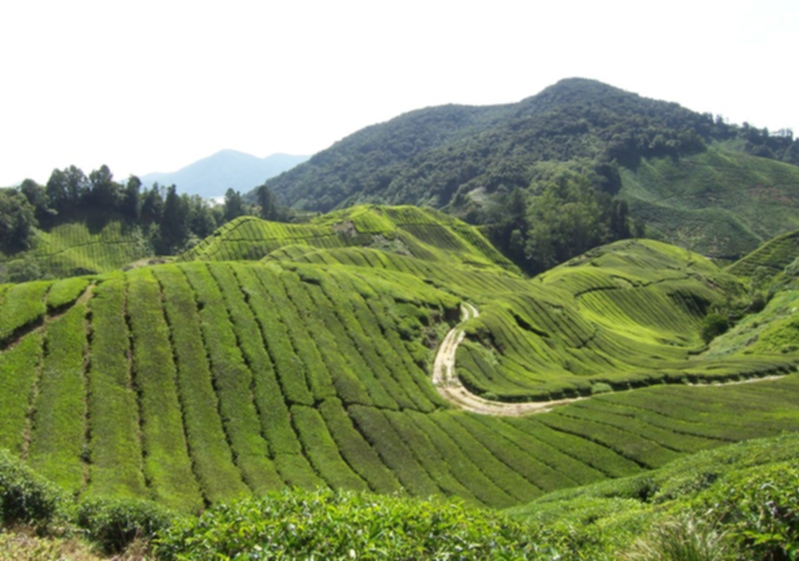
\includegraphics[width=0.382\textwidth]{pictures/tee.JPG}
			\end{center}
			%\caption{A gull}
		\end{wrapfigure}
		
		Unter \definition{Optimierung} versteht man die Festlegung eines bestimmten Programms, mit dessen Hilfe der günstigste Wert für ein vorgegebenes Ziel erreicht wird. Dabei spielen Restriktionen (Nebenbedingungen), die sich oft durch Ungleichungen ausdrücken lassen, eine wichtige Rolle.
		
		Wir betrachten hier verhältnismässig einfache Probleme, die sich mit graphischen Methoden lösen lassen: Von einer Funktion $Z$ (genannt \definition{Ziel\-funk\-tion}) werden extremale Werte bestimmt, wobei die Nebenbedingungen (lineare Ungleichungen) zu beachten sind. Diese Bedingungen ergeben, graphisch in einem Koordinatensystem dargestellt, das sogenannte \definition{Planungspolygon}.
		
		\begin{bsp}
			Eine Fabrik stellt die beiden Modelle \glqq analog\grqq\ und \glqq digital\grqq\ eines Taschenradios her. Jedes Radio der Analogausführung bringt einen Gewinn von Fr. 15.-, das der Digitalausführung Fr. 45.-.
			Die Tagesproduktion der Firma unterliegt den folgenden Einschränkungen: Von der Analogausführung können höchstens 1200, von der Digitalausführung höchstens 700, von beiden zusammen höchstens 1400 Stück hergestellt werden. In der Analogausführung wird eine Verstärkerstufe, in der Digitalausführung werden zwei Verstärkerstufen eingebaut. Pro Tag stehen aber höchstens 1800 Verstärkerstufen zur Verfügung.
			
			Wie viele Analog- bzw. Digitalradios soll die Firma pro Tag herstellen, wenn ihr Gewinn möglichst gross sein soll?
			Werden die Anzahl der pro Tag hergestellten Analoggeräte mit $x$ und die Anzahl der Digitalgeräte mit $y$ bezeichnet, so können die erwähnten Nebenbedingungen (Restriktionen) als ein Ungleichungssystem formuliert werden:
			\begin{align}
				x&\leq1200\\
				y&\leq700\\
				x+y&\leq1400\\
				x+2y&\leq1800
			\end{align}
			Ausserdem gelten noch die Bedingungen
			\begin{align*}
				x\geq0\\
				y\geq0
			\end{align*}
			da ja die Anzahlen $x$ und $y$ nicht negativ sein können.
			
			Zunächst wird das \textbf{Planungspolygon}, die Lösungsmenge des Ungleichungssystems, erstellt:
			\begin{figure}[h!]
				\begin{center}
					\definecolor{zzttqq}{rgb}{0.6,0.2,0}
					\definecolor{cqcqcq}{rgb}{0.75,0.75,0.75}
					\scalebox{1}{
						\begin{tikzpicture}[line cap=round,line join=round, x=0.0033cm,y=0.0033cm]
							\draw [color=cqcqcq,dash pattern=on 3pt off 3pt, xstep=0.66cm,ystep=0.66cm] (-200,-196.58) grid (1920.04,1500);
							\draw[-{Latex[length=8pt, width=8pt]},color=black] (-200,0) -- (1920.04,0);
							\foreach \x in {-200,200,400,600,800,1000,1200,1400,1600,1800}
							\draw[shift={(\x,0)},color=black] (0pt,2pt) -- (0pt,-2pt) node[below] {\scriptsize $\x$};
							\draw[color=black] (1878.85,13.68) node [anchor=south west] { x};
							\draw[-{Latex[length=8pt, width=8pt]},color=black] (0,-196.58) -- (0,1500);
							\foreach \y in {,200,400,600,800,1000,1200,1400}
							\draw[shift={(0,\y)},color=black] (2pt,0pt) -- (-2pt,0pt) node[left] {\scriptsize $\y$};
							\draw[color=black] (12.11,1431.59) node [anchor=west] { y};
							\clip(-200,-196.58) rectangle (1920.04,1500);
							\fill[color=zzttqq,fill=zzttqq,fill opacity=0.1] (1.1,700) -- (400,700) -- (1000,400) -- (1200,200) -- (1200,0) -- (0,0) -- cycle;
							\draw [domain=-200:1920.04] plot(\x,{(--1400-1*\x)/1});
							\draw [domain=-200:1920.04] plot(\x,{(--1800-1*\x)/2});
							\draw [domain=-200:1920.04] plot(\x,{(--700-0*\x)/1});
							\draw (1200,-196.58) -- (1200,1500);
						\end{tikzpicture}
					}
				\end{center}
				\caption{Planungspolygon}
			\end{figure}
			
			Für den Gewinn der Firma in Abhängigkeit von $x$ und $y$ hat man den Funktionsterm
			$$G(x,y)=15x+45y.$$
			$G$ heisst \textbf{Zielfunktion} und ist eine affine Funktion mit 2 Variablen. Alle Paare $(x\mid y)$, die die obigen Bedingungen erfüllen, stellen zulässige Lösungen des Problems dar. Gesucht wird aber dasjenige Paar $(x\mid y)$ ($x,y$ sind natürliche Zahlen), für das der Gewinn $G(x,y)$ maximal wird.
			
			Durch Umformen des Zielfunktionsterms erhält man
			$$y=-\frac{1}{3}x+\frac{G}{45}$$
			eine affine Funktionsschar. Die entsprechende Graphen sind parallele Geraden mit den $y$-Achsenabschnitten $\frac{G}{45}$. Gesucht ist ein Punktepaar $(x\mid y)$, das einerseits das Ungleichungssystem erfüllt, und für das andererseits der y-Achsenabschnitt $\frac{G}{45}$ und damit auch $G$ möglichst gross wird.
			Man erhält die Lösung $(x\mid y)$, indem man eine Gerade der Geradenschar, etwa die durch die Punkte $(0\mid 100)$ und $(300\mid 0)$, $m=-\frac{1}{3}$, auswählt, und sie solange längs der y-Achse nach oben verschiebt, bis sie mit der Begrenzungslinie des Planungspolygons nur noch einen Punkt oder eine Strecke gemeinsam hat.
			\begin{figure}[h!]
				\begin{center}
					\definecolor{zzttqq}{rgb}{0.6,0.2,0}
					\definecolor{cqcqcq}{rgb}{0.75,0.75,0.75}
					\scalebox{1}{
						\begin{tikzpicture}[line cap=round,line join=round, x=0.0033cm,y=0.0033cm]
							\draw [color=cqcqcq,dash pattern=on 2pt off 2pt, xstep=1.32cm,ystep=1.32cm] (-200,-196.58) grid (1920.04,1500);
							\draw[-{Latex[length=8pt, width=8pt]},color=black] (-200,0) -- (1920.04,0);
							\foreach \x in {-200,200,400,600,800,1000,1200,1400,1600,1800}
							\draw[shift={(\x,0)},color=black] (0pt,2pt) -- (0pt,-2pt) node[below] {\scriptsize $\x$};
							\draw[color=black] (1878.85,13.68) node [anchor=south west] { x};
							\draw[-{Latex[length=8pt, width=8pt]},color=black] (0,-196.58) -- (0,1500);
							\foreach \y in {,200,400,600,800,1000,1200,1400}
							\draw[shift={(0,\y)},color=black] (2pt,0pt) -- (-2pt,0pt) node[left] {\scriptsize $\y$};
							\draw[color=black] (12.11,1431.59) node [anchor=west] { y};
							\draw[color=black] (0pt,-10pt) node[right] {\footnotesize $0$};
							\clip(-200,-196.58) rectangle (1920.04,1500);
							\fill[color=zzttqq,fill=zzttqq,fill opacity=0.1] (1.1,700) -- (400,700) -- (1000,400) -- (1200,200) -- (1200,0) -- (0,0) -- cycle;
							\draw [domain=-200:1920.04] plot(\x,{(--1400-1*\x)/1});
							\draw [domain=-200:1920.04] plot(\x,{(--1800-1*\x)/2});
							\draw [domain=-200:1920.04] plot(\x,{(--700-0*\x)/1});
							\draw (1200,-196.58) -- (1200,1500);
							\draw [domain=-200:1920.04] plot(\x,{(--100-0.33*\x)/1});
							\draw[smooth,samples=100,domain=-100.0:1400.0] plot(\x,{300-\x/3});
							\draw[smooth,samples=100,domain=-100.0:1400.0] plot(\x,{500-\x/3});
							\draw[smooth,samples=100,domain=-100.0:1400.0] plot(\x,{835-\x/3});
							\draw[smooth,samples=100,domain=-100.0:1400.0] plot(\x,{700-\x/3});
							\draw[color=black] (-100,80) node {$y_Z$};
						\end{tikzpicture}
					}
				\end{center}
				\caption{Zielgerade und Optimum}
			\end{figure}
			Wie aus der Zeichnung abzulesen ist, entpuppt sich das Paar $(400\mid 700)$ als optimale Lösung des Problems. Die Firma erzielt einen maximalen Gewinn, wenn sie pro Tag 400 Analogradios und 700 Digitalradios herstellt. Den entsprechenden Gewinn berechnet man mit Hilfe der Zielfunktion:
			$$G(400,700) = \unit[15\cdot400]{Fr.} + \unit[45\cdot700]{Fr.} = \unit[37\,500]{Fr.}$$
			Die optimale Lösung kann auch rechnerisch ermittelt werden, indem man den Schnittpunkt der beiden entsprechenden Geraden berechnet (Lösen eines Gleichungssystems mit 2 Unbekannten).
		\end{bsp}
		
		\begin{uebenv}{weidebetrieb}
			Ein landwirtschaftlicher Weidebetrieb hat sich auf die Haltung von
			Kühen und Jungvieh spezialisiert. In den Ställen des Betriebs
			können höchstens $70$ Kühe und $500$ Stück Jungvieh gehalten
			werden.
			
			Für die Ernährung einer Kuh sind $0.25$ ha, für ein
			Jungvieh $0.10$ ha Weideland nötig. Insgesamt hat der Betrieb $50$
			ha Weideland.
			
			Für die Pflege der Kühe und des Jungviehs stehen drei
			Arbeiter zur Verfügung, die insgesamt $8000$ Arbeitsstunden im
			Jahr leisten. Für eine Kuh sind $100$ Arbeitsstunden, für ein
			Stück Jungvieh $10$ Arbeitsstunden je Jahr notwendig. Der Gewinn
			bei einer Kuh beträgt $\unit[400]{Franken}$, bei einem Jungvieh $\unit[50]{Franken}$ im
			Jahr.
			
			Wie viele Kühe und wie viel Stück Jungvieh muss der
			Betrieb halten, damit der Gesamtgewinn möglichst gross wird?
		\end{uebenv}
		
		\subsection{Regeln zum Lösen von Aufgaben zur linearen Optimierung}
		Eine Aufgabe zur linearen Optimierung löst man wie folgt:
		
		\begin{enumerate}
			\item Annahme:
			\begin{itemize}
				\item Man stellt die gegebenen Daten tabellarisch dar
				\item und definiert die Unbekannten.
			\end{itemize}
			\item Ungleichungen:
			\begin{itemize}
				\item Man übersetzt die im Aufgabentext umschriebenen
				Bedingungen in die Formelsprache der Mathematik.
			\end{itemize}
			\item Planungspolygon:
			\begin{itemize}
				\item Man stellt die Lösungen des Ungleichungssystems graphisch
				dar.
			\end{itemize}
			Dabei verwendet man folgende Tatsachen:
			\begin{itemize}
				\item Punkte, deren Koordinaten $(x\mid y)$ die Ungleichung $y>mx+b$
				bzw. $y<mx+b$ erfüllen, bilden eine Halbebene, die oberhalb bzw.
				unterhalb des Graphen der Funktion $y=mx+b$ liegt.
				\item Der mengentheoretische Durchschnitt aller Halbebenen, die
				sich aus den Ungleichungen ergeben, bilden das sogenannte
				Planungspolygon.
			\end{itemize}
			
			\item Zielfunktion:
			\begin{itemize}
				\item Man drückt die Grösse $z$, die optimal werden soll, mit
				den Unbekannten aus.
				\item Man löst die Gleichung nach $y$ auf
				\item und zeichnet den zugehörigen Graphen für ein frei
				wählbares $z$ im gleichen Koordinatensystem wie das
				Planungspolygon ein.
			\end{itemize}
			\item Optimum:
			\begin{itemize}
				\item Man untersucht, welche Parallele zur Zielgerade das
				Planungspolygon in mindestens einem Punkt $P$ schneidet und ein
				optimales $z$ liefert.
				\item $P$ ist der optimale Punkt; man berechnet seine
				Koordinaten.
				\item Falls die Koordinaten von $P$ nicht ganze Zahlen sind, die
				gesuchten Unbekannten jedoch ganzzahlig sein sollten, muss man
				die Umgebung von $P$ in einer zusätzliche Skizze vergrössert
				darstellen, damit man gegebenenfalls richtig runden kann.
			\end{itemize}
			\item Antwort:
			\begin{itemize}
				\item Man liest die Aufgabenstellung erneut.
				\item Man beantwortet die gestellten Fragen mit einem Text.
			\end{itemize}
			
		\end{enumerate}

\clearpage

\subsection{Notizen zu den Übungen}

\begin{lsg}{weidebetrieb}
<<<<<<< Updated upstream
			Die Zielfunktion ist $z(x)=400x+50y\Leftrightarrow y_z=-8x+\frac{z}{50}$ und die Bedingungen
=======
			Die Zielfunktion ist $z(x,y)=400x+50y\Leftrightarrow y_z=-8x+\frac{z}{50}$ und die Bedingungen
>>>>>>> Stashed changes
			\begin{align}
				0.25x+0.1y\leq50 &\Leftrightarrow y_1\leq -2.5x+500\\
				100x+10y\leq8000 &\Leftrightarrow y_2\leq -10x+800
			\end{align}
			Das Planungspolygon sieht so aus:
			
			\begin{center}
				\begin{tikzpicture}[xscale=0.1,yscale=0.012]
					% Achsen zeichnen
<<<<<<< Updated upstream
					\draw[-{Latex[length=8pt, width=8pt]}] (-10,0) -- (80,0) node[right] {$x$};
					\draw[-{Latex[length=8pt, width=8pt]}] (0,-50) -- (0,500) node[above] {$y$};
=======
					\draw[-{Latex[length=8pt, width=8pt]}] (-7,0) -- (80,0) node[right] {$x$};
					\draw[-{Latex[length=8pt, width=8pt]}] (0,-50) -- (0,520) node[above] {$y$};
>>>>>>> Stashed changes
					
					% Skala auf der x-Achse
					\foreach \x in {10,20,...,70} \draw (\x,3pt) -- (\x,-3pt) node[below] {\x};
					
					% Skala auf der y-Achse
					\foreach \y in {0,100,...,500} \draw (3pt,\y) -- (-3pt,\y) node[left] {\y};
					
					% Gitter zeichnen
<<<<<<< Updated upstream
					\draw[very thin, lightgray] (-5,-10) grid[xstep=10, ystep=100] (75,550);
=======
					\draw[very thin, lightgray] (-5,-8) grid[xstep=10, ystep=100] (75,530);
>>>>>>> Stashed changes
					
					% Gerade y1 = -2.5x + 500
					\draw[domain=-5:75, smooth, variable=\x, blue] plot ({\x}, {-2.5*\x + 500}) node[right] {$y_1 = -2.5x + 500$};
					
					% Gerade y2 = -10x + 800
					\draw[domain=25:75, smooth, variable=\x, red] plot ({\x}, {-10*\x + 800}) node[right] {$y_2 = -10x + 800$};
					
					% Gerade y = 500
					\draw[domain=-5:75, smooth, variable=\x, seagreen] plot ({\x}, {500}) node[right] {$y = 500$};
					
					% Gerade x = 70
					\draw[domain=-20:535, smooth, variable=\y, orange] plot ({70}, {\y}) node[above] {$x = 70$};
					
					% Gerade yz = -8x + 300
<<<<<<< Updated upstream
					\draw[domain=-3:55, smooth, variable=\x, purple] plot ({\x}, {-8*\x + 350}) node[right] {$y_z = -8x + 300$};
=======
					\draw[domain=-3:55, smooth, variable=\x, purple] plot ({\x}, {-8*\x + 350}) node[right] {$y_z = -8x + Z$};
>>>>>>> Stashed changes
				\end{tikzpicture}
			\end{center}
			
			$z$ soll möglichst gross werden. Der Punkt, der noch im Planungspolygon liegt und $z$ maximiert muss der Schnittpunkt der Geraden $y_1$ und $y_2$ sein, da die Steigung $-8$ zwischen den Steigungen $-2.5$ und $-10$ liegt. Aus $y_1=y_2$ folgt $x=40$ und damit $y=400$. Also resultiert optimaler Gewinn, wenn man $40$ Kühe und $400$ Rinder hält.
		\end{lsg}
		
		\clearpage
		\listoffigures
		%\listoftables
		%\newpage
		%\nocite{*}
		%\bibliographystyle{plain}
		%\bibliography{preamble/literaturgoogle}
	\end{document}